\subsection{В элементарной теории вещественных чисел}
\setauthor{Егор Суворов}

\subsubsection{Мотивация}
	\begin{assertion}
		Элиминация кванторов возможна в следующей арифметике над $\R$:
		$\mathcal P = \{=, >\}$, $\mathcal F = \{+, \cdot, 0, 1\}$.
	\end{assertion}
	\begin{Rem}
		$x > 0$ не выразить бескванторной формулой в $(\R, =, +, x, 0, 1)$
	\end{Rem}
	\begin{Rem}
		Если разрешать любые формулы, то 0 и 1 не нужны, да и $>$ тоже:
		\begin{itemize}
		\item $x = 0 \iff \forall y \colon x + y = x$
		\item $x = 1 \iff \forall y \colon x \cdot y = x$
		\item $x > y \iff \exists z \colon x = y + z ^ 2$.
		\end{itemize}
	\end{Rem}

	Как вообще выглядят атомарные формулы?
	Всего два вида: $P(x_1, \dots, x_n)=0$ или $P(x_1, \dots, x_n) > 0$, где $P$ "--- многочлен с целыми коэффициентами.
	Обращаем внимание, что если добавить рациональные константы, то ничего бы не изменилось "--- многочлен всегда можно домножить на общий знаменатель
	и получить многочлен с целыми коэффициентами.

	Далее будет рассказан алгоритм, который не слишком эффективен (и вообще плохо оценивается по скорости).
	Лучший результат в этой области оценивается как двойная экспонента ($2^{2^n}$), при этом есть нижняя оценка того же порядка.

	Что вообще нам даст элиминация кванторов алгоритмом?
	Можно любую формулу в элементарной теории вещественных чисел проверить: свести к бескванторной форме, а потом просто подставить.

	\begin{exmp}
	Любую задачу школьной геометрии, где используются только прямые, окружности (и их куски),
	которые касаются и пересекаются, можно записать в координатах, получить какой-то набор условий
	в арифметике, а потом алгоритмически доказать или проверить.
	\end{exmp}

	\begin{exmp}
	В школе учат элиминировать кванторы в выражении вида $\exists x \colon (x^2 + px + q = 0)$.
	Это просто условие на существование решения квадратного уравнения, можно записать бескванторно: $p^2-4q \ge 0$ (условие на дискриминант).
	Для уравнений б\'ольшей степени в школе обычно не изучают, однако из того, что мы сейчас докажем,
	следует, что для любых уравнений и неравенств подобные эквивалентности существуют.
	\end{exmp}

\subsubsection{Основные определения}
	Будет рассказан так называемый алгоритм Тарского (Тарского-Зайденберга).
	Изначальная версия была сложной, но есть более простая:
	\begin{theorem}[Тарского-Зайденберга]\label{tarski_seidenberg}
		В $(\R, =, >, +, \cdot, 0, 1)$ допустима элиминация кванторов.
	\end{theorem}

	\begin{Def}
		Алгебраическое множество "--- это решение системы уравнений из многочленов.
	\end{Def}

	\begin{Def}
		Полуалгебраическое множество в $\R^n$ "--- это объединение конечного числа
		множеств решений систем полиномиальных уравнений и неравенств.
	\end{Def}
	\begin{Rem}
		Например:
		\[
			\left[
			\begin{array}{l}
				\begin{cases}
					xy+y^5 - 20 = 0 \\
					z^2 - 3 = 0 \\
					x + y \ge 0 \\
				\end{cases}\\
				\begin{cases}
					xy+y^5 - 20 = 0 \\
					z^2 = 3 \\
					z^{100} \le x
				\end{cases}
			\end{array}
			\right.
		\]
	\end{Rem}
	\begin{Rem}
		Чуть более строго: алгебраическое множество "--- это множество таких $\vec x$, для которых выполняется некоторое условие следующего вида:
		\[ \Lor_i \Land_j P_{ij}(\vec x) \begin{smallmatrix}>\\=\end{smallmatrix} 0 \]
		Здесь $P_{ij}$ "--- многочлены от многих переменных с целыми коэффициентами.
	\end{Rem}

	\begin{assertion}
		Объединение полуалгебраических множеств тоже полуалгебраическое.
	\end{assertion}
	\begin{proof}
		Очевидно: просто объединяем две дизъюнкции.
	\end{proof}

	\begin{Exercise}
		Пересечение полуалгебраических множеств полуалгебраично.
	\end{Exercise}
	\begin{proof}
		Подсказка: надо взять конъюнкцию условий, а дальше раскрыть скобки по дистрибутивности.
		Условно, привести в ДНФ.
	\end{proof}

	\begin{assertion}
		Любое полуалгебраическое множество задаётся некоторой бескванторной формулой.
	\end{assertion}
	\begin{proof}
		Это очевидно: формулу без кванторов (но с многочленами) мы можем написать по определению, а многочлены "--- вполне себе бескванторные формулы.
	\end{proof}

	\begin{assertion}
		Любая бескванторная формула задаёт полуалгебраическое множество.
	\end{assertion}
	\begin{proof}
		Сначала избавимся от отрицания:
		\begin{enumerate}
			\item $\lnot (a = b) \longrightarrow (a < b) \lor (a > b)$
			\item $\lnot (a > b) \longrightarrow (a = b) \lor (a < b)$
		\end{enumerate}
		Приводим в ДНФ (алгоритмом раскрытия скобок, при котором отрицаний не возникает).
		Получаем в точности определение полуалгебраического множества.
	\end{proof}

\subsubsection{Проеция полуалгебраического}
	\begin{assertion}\label{semialg_proj}
		Проекция полуалгебраического множества из $\R^{n+1}$ вдоль оси координат является полуалгебраическим множеством в $\R^n$.
	\end{assertion}
	\begin{exmp}
		Пусть было полуалгебраическое множество $A$ в $\R^3$, задающее <<шапку>> сферы:
		\[ (x^2+y^2+z^2 = 1) \land \left(z > \frac 1 2\right) \]
		Тогда мы можем спроецировать $A$ вдоль оси $OZ$, получить некоторое множество $B$ на плоскости $OXY$.
		Нетрудно понять, что это на самом деле круг, то есть тоже полуалгебраическое множество:
		\[ x^2 + y^2 < \frac{3}{4} \]
	\end{exmp}
	\begin{Rem}
		Утверждение \ref{semialg_proj} эквивалентно \hyperref[tarski_seidenberg]{теореме Тарского-Зайденберга}.
	\end{Rem}
	\begin{proof}
		Если теорема верна, то утверждение очевидно: это просто навешивание снаружи квантора существования по оси.

		В другую сторону: можно заменить кванторы $\forall$ на $\exists$ и запустить индукцию по числу кванторов (как обычно).
		Пусть была формула с кванторами существования, взяли самый внутренний: $\exists x_i \colon F$, причём $F$ бескванторна.
		Тогда $F$ полуалгебраическое, а по утверждению его проекция, т.е. множество $\exists x_i \colon F$ "--- полуалгебраическое,
		т.е. можно переписать этот кусок формулы без кванторов, что и требовалось доказать для перехода в индукции.
	\end{proof}

	Основная идея доказательства: метод интервалов из школьной программы.
	\begin{exmp}
		В школе рассказывают метод интервалов: найти, где какой знак имеет следующий многочлен:
		\[ (x-1)^2(x-3)(x+5)>0 \]
		На бесконечности многочлен имеет знак плюс, в корнях знак как-то меняется,
		Давайте нарисуем корни на числовой прямой.
		Свели бесконечное число разных $x$ к лишь конечному числу случаев:
		\begin{center}
			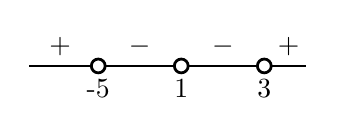
\begin{tikzpicture}[x=0.1em,y=0.1em,line width=0.1em]
			\draw (25, 0) circle [radius=2.5];
			\draw (55, 0) circle [radius=2.5];
			\draw (85, 0) circle [radius=2.5];
			\node at (25, -8) {-5};
			\node at (55, -8) {1};
			\node at (85, -8) {3};
			\draw (0, 0) -- node[above] {$+$} (22.5, 0);
			\draw (27.5, 0) -- node[above] {$-$} (52.5, 0);
			\draw (57.5, 0) -- node[above] {$-$} (82.5, 0);
			\draw (87.5, 0) -- node[above] {$+$} (100, 0);
			\end{tikzpicture}
		\end{center}
	\end{exmp}

	Теперь давайте избавляться от квантора существования в общем случае.
	Есть формула:
	\[ \exists x \colon \phi(x, x_1, \dots, x_n) \]
	Мы считаем, что все атомарные формулы имеют вид $P_i(x, x_1, \dots, x_n) \begin{smallmatrix}>\\=\end{smallmatrix} 0$.
	Будет удобно считать, что у нас на самом деле многочлен от одной переменной $x$,
	а вот коэффициенты при степенях "--- многочлены от $x_1, \dots, x_n$.
	По сути следующая замена:
	\[ \Z[x, x_1, \dots, x_n] = \Z[x_1, \dots, x_n][x] \]
	Выпишем все многочлены из $\Z[x, x_1, \dots, x_n]$, которые встретились в атомарных формулах: $P_1, \dots, P_k$.
	Заметим, что если мы подставим $x_1=a_1, x_2=a_2, \dots$ ($a_i \in \R$), то у нас все этим многочлены $P_i$ станут многочленами от $x$.

\subsubsection{Диаграммы}
	Пусть $Q_1, \dots, Q_k$ "--- многочлены от одной переменной.
	(нас будут интересовать те, которые получились из $P_k$, но вообще сейчас на это опираться не будем).
	\begin{Def}
		Пусть $\alpha_1, \alpha_2, \dots, \alpha_n$ "--- это все различные корни ненулевых многочленов, причём в порядке возрастания.
		Диаграммой для многочленов называется некоторая табличка из $k$ строк и $2n+1$ столбцов.
		Рисуем про каждый интервал между соседними корнями (и в корнях тоже) нули, плюсы, минусы:
		\[
		\begin{array}{|c|c|c|c|c|c|c|c|}
		\hline
		& \dots & \alpha_1 & \dots & \alpha_2 & \dots\dots\dots & \alpha_n & \dots \\\hline
		Q_1 & \sign Q_1(-\infty) & \sign Q_1(\alpha_1) & \sign Q_1(\frac{\alpha_1+\alpha_2}{2}) & \sign Q_1(\alpha_2) & \dots\dots\dots & \sign Q_1(\alpha_n) & \sign Q_1(+\infty) \\\hline
		\vdots & \vdots & \vdots & \vdots & \vdots & \ddots & \vdots & \vdots \\\hline
		Q_k & \sign Q_k(-\infty) & \sign Q_k(\alpha_1) & \sign Q_k(\frac{\alpha_1+\alpha_2}{2}) & \sign Q_k(\alpha_2) & \dots\dots\dots & \sign Q_k(\alpha_n) & \sign Q_k(+\infty) \\\hline
		\end{array}
		\]
		Причём в диаграмму список корней и многочленов \textit{не входят}.
		Однако порядок многочленов при этом фиксирован, то есть переставлять строки диаграммы нельзя (не говоря уже о столбцах).
	\end{Def}
	\begin{exmp}
		Пусть есть многочлены $x^2-1$, $x$, $0$, у них корни $-1, 0, 1$.
		\[
		\begin{array}{|c|c|c|c|c|c|c|c|}
		\hline
		      & \dots & -1 & \dots & 0 & \dots & 1 & \dots \\\hline
		x^2-1 & +     & 0  & -     & - & -     & 0 & +     \\\hline
		x     & -     & -  & -     & 0 & +     & + & +     \\\hline
		0     & 0     & 0  & 0     & 0 & 0     & 0 & 0     \\\hline
		\end{array}
		\]
		Так как ни корни, ни многочлены не входят в диаграмму, для $x^2-4$, $2x$, $0$ диаграмма получилась бы такая же.
	\end{exmp}

	\begin{Rem}
		Имея диаграмму для многочленов $P_i$ с подставленными $x_1, \dots$ легко определить истинность логической формулы, потому что мы знаем вообще все возможные варианты знаков,
		которые бывают у многочленов при фиксированных $x_1, \dots$ и произвольном $x$.
		Мы просто перебираем конечное число вариантов, подставляем в логическую формулу, вычислили значение формулы.
	\end{Rem}

	\begin{assertion}\label{fix_diag_semialg}
		Множество таких $(a_1, \dots, a_n) \in \R^n$, что при подстановке $x_1=a_1, \dots, x_n=a_n$ получается некоторая фиксированная диаграмма, является полуалгебраическим.
	\end{assertion}
	\begin{Rem}
		Если докажем, то докажем и утверждение \ref{semialg_proj}.
		В самом деле: вспомним про многочлены $P_i$.
		При разных подстановках $x_1, \dots, x_n$ у нас получаются разные наборы многочленов $Q_i(x)$, эти наборы дают разные диаграммы.
		Диаграмм конечно и ограничено "--- количество столбцов не больше количества корней у всех многочленов $Q_i(x)$ (то есть не больше суммарной степени по $x$ у $P_i$),
		количество строк тоже ограничено (не более, чем у нас $P_i$), в каждой ячейке диаграммы "--- одно значение из трёх.

		Тогда для бескванторного выражения проекции можно просто перебрать все диаграммы, из них выбрать те, которые нас устраивают (т.е. есть корректный столбец),
		для каждой диаграммы узнать, какие подстановки $x_1, \dots, x_n$ нам дадут нужную диаграмму "--- это что-то полуалгебраическое.
		Потом просто объединяем все такие полуалгебраические.
	\end{Rem}
	\begin{Rem}
		Другое объяснение: у нас есть $\R^n$ (то, куда проецируем), оно разбилось на какие-то куски, в каждом куске "--- ровно одна диаграмма.
		Некоторые диаграммы годятся (т.к. обращают логическую формулу в истину), а некоторые "--- нет.
		Ответ, который мы хотим найти "--- объединение всех годных диаграмм.
	\end{Rem}

\subsubsection{Доказательство утверждения \ref{fix_diag_semialg}}	
	Идея: нам будет удобно \textit{добавлять} лишние многочлены.
	\begin{assertion}
		Пусть мы доказали, что для конкретных многочленов $P_1, \dots, P_{k+1}$ (лежащих в $\Z[x, x_1, \dots, x_n]$) и любой диаграммы
		у нас множество соответствующих подстановок переменных $x_1, \dots, x_n$ полуалгебраическое.
		Тогда, выкинув $P_{k+1}$, мы тоже получим, что для любой диаграммы множество допустимых подстановок "--- полуалгебраическое.
	\end{assertion}
	\begin{proof}
		Перебрали все диаграммы для $k+1$ многочлена, выкинули строчку для многочлена $P_{k+1}$, получили какую-то диаграмму для $P_1, \dots, P_k$.
		Тогда получается, что для каждой диаграммы набора $P_1, \dots, P_k$ искомое множество есть объединение некоторых множеств,
		соответствующих каким-то диаграммам расширенного набора многочленов (такие множества полуалгебраические), т.е.
		искомое множество тоже полуалгебраическое.
	\end{proof}

	Теперь вопрос: как мы будем добавлять многочлены и какие, чтобы стало проще?
	Будем \textit{насыщать} наше множество.
	Вспомним, что мы можем многочлены $P$ записывать, как многочлены от $x$ с коэффициентами из $\Z[x_1, \dots, x_n]$ и
	введём операции, которые добавляют что-то в текущее множество многочленов:
	\begin{enumerate}
	\item
		Взятие старшего члена: был многочлен
		\[ P = Q_1x^n + Q_2x^{n-1} + \dots \]
		Добавляем многочлен $Q_1(x_1, \dots, x_n)$, не зависящий от $x$.
	\item
		Вычёркивание старшего члена: был многочлен
		\[ P = Q_1 x^n + Q_2 x^{n-1} + \dots + Q_{n+1} \]
		добавили многочлен
		\[ Q_2 x^{n-1} + \dots + Q_{n+1} \]
	\item
		Формальная производная $P$ по переменной $x$: $\partd{P}{x}$:
		\begin{gather*}
		Q_1x^n + Q_2x^{n-1} + \dots \\
		\downarrow \\
		(nQ_1)x^{n-1} + ((n-1)Q_2)x^{n-2} + \dots
		\end{gather*}
	\item
		Модифицированный остаток от деления $P$ на $Q$ (напоминаем, что $P, Q \in \Z[x_1, \dots, x_n][x]$).
		Это просто обычный остаток от деления (как многочленов с переменной $X$), но дополнительно домноженный на старший коэффициент $Q$ в большой степени,
		чтобы не вылезти из кольца многочленов с \textsl{целыми} коэффициентами.
		\[ Q = r_1(x_1, \dots, x_n) x^m + \dots \]
		Мы берём $(p \bmod Q) \cdot r_1 ^ C$, где $C$ "--- константа, зависящая от $P$ и $Q$.
		Давайте брать такую минимальную константу, чтобы получился многочлен.
	\end{enumerate}
	Давайте насытим множество многочленов относительно операций 1--4.
	То есть берём и применяем операции как угодно, пока получаются новые многочлены.
	\begin{assertion}
		Этот процесс остановится через конечное число шагов
	\end{assertion}
	\begin{proof}
		Будет на следующей лекции.
		\TODO
	\end{proof}

	Пусть $F_0$ "--- это многочлены степени ноль (по $x$) из насыщенного множества $A$.
	То есть это все многочлены вида $P(x_1, \dots, x_n)$, не зависящие от $x$.
	Тогда утверждается, что диаграмма для $F_0$ (которая будет состоять из одного столбца и, понятное дело,
	соответствующие значения $x_1, \dots, x_n$ являются полуалгебраическим множеством "--- просто пишем условия на $P$'шки)
	позволяет однозначно восстановить диаграмму для исходного $A$.

	Воссстанавливаем диаграмму индукцией по степени.
	Для степени $0$ всё есть по условию, теперь пусть у нас есть диаграмма для многочленов степени $\le k$.
	Добавляем какой-то многочлен $P$ степени $k+1$.
	\begin{enumerate}
	\item
		Посмотрели на строчку, соответствующую старшему коэффициенту $P$ (помним, что коэффициенты $P$ "--- это многочлены).
		Если в ней везде нули, то надо просто повторить строчку для многочлена $P$ без старшего коэффициента (такой у нас в диаграмме есть).
		Например, везде нули могли получиться, если у нас особо удачные $a_i$, зануляющие старший коэффициент $P$.
		Если же нули не везде, то надо сделать следующее:
	\item
		Посчитать значение в старых корнях.
		Взяли старый корень $\alpha$ многочлена $Q$, поделили $P$ с остатком (модифицированным) на $Q$,
		получили $R+Q\cdot (\dots)=P\cdot \beta^C$ (тут $\beta$ "--- старший коэффициент $P$, а $C$ "--- константа).
		Тогда $Q\cdot (\dots)$ занулился, знак $R$ у нас есть, надо его, возможно, поменять (так как знак $\beta$ есть, $C$ есть)
	\item
		Добавить новые корни $P$ (в них значение "--- ноль).
		Кратные корни "--- это корни производной, поэтому они уже есть.
		Размышление: если у нас в какой-то строчке получилось \t{+-} или \t{-+}, то надо добавить между ними корень.
		Значение корня нам в целом неважно, важен порядок.
		Утверждение: случаев вроде <<\t{++} и надо добавить чётное число корней>> или <<\t{+-}, надо добавить больше одного корня между ними>> не бывает,
		так как по теореме Ролля между любыми двумя корнями есть корень производной.
	\item
		Осталось вычислить промежуточные значения.
		На плюс бесконечности значение определяется знаком старшего коэффициента.
		Дальше, когда мы переходим через какой-то корень, в нём либо $P$ не ноль (тогда знак не меняется),
		либо ноль (тогда надо понять кратность) и знак может как поменяться, так и не поменяться.
		Кратность $P$ в точке считается методом <<взяли много производных, посмотрели сколько из них подряд занулилось>>.
	\item
		А у старых многочленов новые точки и промежутки просто вложены в старые промежутки и однозначно продлевается.
	\end{enumerate}
